\documentclass[a4,english]{report}
\usepackage[a4paper, hmargin=2.5cm,vmargin=1.5cm]{geometry}
\usepackage[colorlinks = true]{hyperref}
\hypersetup{
  pdftitle    = {Master thesis - Feedback on Backpressure},
  pdfauthor   = {Richard van Heest},
  colorlinks  = true,
  linkcolor   = [rgb]{0.1,0.1,0.4},
  citecolor   = [rgb]{0.4,0.1,0.1},
  filecolor   = [rgb]{0.1,0.4,0.4},
  urlcolor    = [rgb]{0.1,0.1,0.7}
}
\usepackage{listings}
\usepackage{color}
\usepackage{verbatim} % \verb{} for inline code
\usepackage[numbers,square,sort]{natbib} % references as [1,2,3] in superscript -> see also http://merkel.zoneo.net/Latex/natbib.php
\usepackage{xspace} % put a space after an abbreviation in a newcommand
\usepackage{amsmath}
\usepackage{graphicx} % to show images
\usepackage{float} % places the images at precisely the location in the LaTeX code
\usepackage[bottom]{footmisc} % fix \footnote{} position at the bottom of the page

\newcommand{\todo}[1]{\textcolor{red}{\textbf{\large @TODO: #1}}}
\newcommand{\code}[1]{\sloppy{\mbox{\texttt{#1}}}}
\newcommand{\HRule}{\rule{\textwidth}{0.5mm}}

\newcommand{\obs}{\texttt{Observable}\xspace}
\newcommand{\obv}{\texttt{Observer}\xspace}
\newcommand{\subs}{\texttt{Subscription}\xspace}
\newcommand{\subj}{\texttt{Subject}\xspace}
\newcommand{\bsubj}{\texttt{BehaviorSubject}\xspace}
\newcommand{\ier}{\texttt{IEnumerator}\xspace}
\newcommand{\ieb}{\texttt{IEnumerable}\xspace}
\newcommand{\id}{\texttt{IDisposable}\xspace}

\definecolor{pgreen}{rgb}{0,0.5,0}
\definecolor{pgrey}{rgb}{0.5,0.5,0.5}
\definecolor{mauve}{rgb}{0.58,0,0.82}
\lstdefinestyle{ScalaStyle}{
  frame=tb,
  language=Scala,
  showspaces=false,
  showtabs=false,
  breaklines=true,
  showstringspaces=false,
  breakatwhitespace=true,
  commentstyle=\color{pgreen},
  keywordstyle=\color{blue},
  stringstyle=\color{mauve},
  basicstyle=\ttfamily,
  moredelim=[il][\textcolor{pgrey}]{$$},
  moredelim=[is][\textcolor{pgrey}]{\%\%}{\%\%},
  numbers=left,
  numberstyle=\color{pgrey},
  columns=flexible,
  mathescape=true,
  escapechar=|
}
\lstdefinestyle{HaskellStyle}{
  frame=tb,
  language=Haskell,
  showspaces=false,
  showtabs=false,
  breaklines=true,
  showstringspaces=false,
  breakatwhitespace=true,
  commentstyle=\color{pgreen},
  keywordstyle=\color{blue},
  stringstyle=\color{mauve},
  basicstyle=\ttfamily,
  moredelim=[il][\textcolor{pgrey}]{$$},
  moredelim=[is][\textcolor{pgrey}]{\%\%}{\%\%},
  numbers=left,
  numberstyle=\color{pgrey},
  columns=flexible,
  mathescape=true,
  escapechar=|,
  deletekeywords={return, flip}
}

\begin{document}
\begin{titlepage}
\begin{center}
\textsc{\Large Delft University of Technology}\\[0.5cm]
\textsc{\LARGE Master thesis}\\[0.5cm]
{\huge \bfseries \todo{title of the thesis here}}

\HRule \\[3.0cm]

\begin{tabular}{l r}
	\begin{minipage}{0.5\textwidth}
	\begin{flushleft}
	\large
	\emph{Author:}\\
	Richard \textsc{van Heest} (std. nr. 4086570)\\
	\end{flushleft}
	\end{minipage}
	&
	\begin{minipage}{0.464\textwidth}
	\begin{flushright}
	\large
	\emph{Thesis committee:}\\
	Prof. dr. H.J.M. \textsc{Meijer}\\
	\todo{other members of the thesis committee here}
	\end{flushright}
	\end{minipage}
\end{tabular}

\vfill
\textsc{\large \today}

\todo{TU Delft ( + logo), EEMCS, [Master Program], [Chosen Specialization]}\\
\todo{Applied Duality???}
\end{center}
\end{titlepage}

\pagestyle{plain}
\pagenumbering{roman}
\setcounter{page}{1}
\chapter*{Preface}

\todo{content here}
\itemize
	\item Explain the topic and context (institute/company)
	\item Main findings in a few lines
	\item Names of the members of the thesis committee
	\item Acknowledgements
	\item Finish with ‘name’ and ‘date’

\begin{flushright}
Richard van Heest\\
\emph{Middelharnis, January 2016}
\end{flushright}

\clearpage
{\hypersetup{linkcolor = black} \tableofcontents}

\clearpage
\setcounter{page}{1}
\pagenumbering{arabic}
\chapter*{Introduction}
\addcontentsline{toc}{chapter}{Introduction}

Reactive programming is a paradigm in which the program observes events that occur in its environment and reacts to these events as they occur. This is in contrast to the more familiar interactive program flow in which a program \emph{requests} some form of data and only continues the program flow once this data is received. Instead of pulling data in the usual interactive way, reactive programs get data (or events) pushed to them on which they respond according to the program. Some of the most common usages of reactive programming can be found in user interfaces (mouse moves, key events or button presses), network communication, database queries and clocks or timers \cite{meijer2012-YMIAD}.

In an interactive program, the \textit{consumer} is in charge of requesting the data. The \textit{producer} only has to obey the commands from the consumer and return the requested data. In reactive programs this is the exact opposite: the producer is in charge and sends the data \emph{at its own pace} \cite{berry1991-Reactive}, whereas the consumer has to react to the data it receives from the producer.

This shift in roles between producer and consumer poses an interesting problem: ``\textit{What happens when the consumer cannot keep up with the amount of data that is sent by the producer?}''. In other words, when a consumer has to deal with an overproducing source, how can it handle the excessive amount of data? Several solutions with different policies have already been proposed and implemented in order to solve this problem \cite{RxJava-Wiki-Callstack-Blocking,RxJava-Wiki-Backpressure,Reactive-Streams}. We find, however, that some of these work well under certain circumstances but are not suitable for all kinds of reactive programs in general. Other solutions change the contract of reactive programming and put the consumer back into command, but, surprisingly, still call it `reactive'.

This poses the question whether the concepts behind reactive programming have been generalized too much and whether distinctions between different kinds of reactive programs can lead to a clearer view of what solution works best under which conditions. This thesis will discuss this topic extensively in \Cref{chap:problem-statement} and \Cref{chap:exploring-the-problem-space}.

Based on the conclusions of this first part, we will propose a new solution to the overproduction problem, which makes use of control theory and feedback control systems. This solution can be used as a replacement to solutions that put the consumer back in charge.

Feedback control is a technique that is mainly used in mechanical and electrical engineering, but is generally overlooked in computer science. Feedback control can be applied by continuously measuring a system's property, comparing it to a desired value and alter the system's input based on the error between the desired and measured values. The goal is to ultimately bring the measured property as close to the desired value as possible and keep it this way despite external changes that try to bring the system out of balance \cite{janert2013-feedback}.

Although well suited in several use cases, control theory is generally overlooked in computer science and software engineering. To the best of our knowledge, there are even no well-written libraries that allow software developers to construct and run feedback systems in a clean way. As we will use feedback control in our solution for the overproduction problem, we will study the composition of feedback systems in \Cref{chap:intro-to-feedback-control} and present an concise but powerful library for this purpose that is based on the concepts of functional and reactive programming (\Cref{chap:feedback-api}). Using this library, we will then propose our solution to the overproduction problem.

\section*{Research Questions}
\addcontentsline{toc}{section}{Research Questions}
This thesis answers a number of questions that are related to reactive programming, overproducing sources in a reactive context and feedback control, which are listed and briefly introduced in this section.

\subsubsection*{In what ways can a reactive program already be controlled to prevent overproduction?}
There are multiple solutions for controlling overproduction in the context of reactive programming. To understand these solutions we first need to identify the various types of reactive programs and consider their mutual similarities and differences. This is important since the existing solutions do not work for every type of reactive program.

\subsubsection*{How can we implement a \emph{reactive} feedback system that is composed of smaller parts?} 
As the solution to overproduction that is presented in this thesis makes use of control theory and feedback control, and given that these are not yet widely known or used in computer science, it is important to develop an understanding of these techniques and create the tools necessary to construct feedback systems in an easy way. We will show that these can be seen as reactive programs and implement a library on top of existing reactive programming API's.

\subsubsection*{How can the overproduction problem be reduced to a feedback control problem?}
To solve overproduction using feedback control, it is necessary to get out of the context of reactive programming and abstract this into more general problems that can be solved by control theory. Once we develop and solve this more general problem, we can put it back into the context of reactive programs.

\subsubsection*{Can this new solution to overproduction be integrated in an existing API for reactive programming?}
In order for this solution to be useful in practice it is important to be able to interface with existing API's for reactive programming. To test this, a clean API is needed that does not yet implement any solutions for overproduction. For this purpose we use the newly created RxMobile API \cite{RxMobile}.

\section*{Outline}
\addcontentsline{toc}{section}{Outline}
In the next chapter we will continue this thesis report with a short discussion on the definitions of interactive and reactive programming as it is defined in literature (\Cref{chap:problem-statement}). This is followed up with an extensive introduction to a widely used reactive programming API whose concepts have been implemented in many languages. We will discuss the basic principles of this API as well as it's derivation from and relationships with interactive programming interfaces. Once these foundations are laid out, we will give an overview of the different ways in which it tries to overcome overproduction problems. It is important to first gain a good understanding of reactive programming in general and this API especially, since we will build on top of these in the rest of this thesis.

Different circumstances require different approaches to overproduction, as we already hypothesized above. In \Cref{chap:exploring-the-problem-space} we will explore and categorize these circumstances and describe how overproduction is currently best dealt with in each of these situations. Here we also discuss the current state of abstraction over reactive programming and describe our solution to overproduction and explain for which type of reactive programs we think this will apply.

As we will use control theory to solve the problem of overproduction, and given that this topic is not well known in computer science we will briefly introduce this topic in \Cref{chap:intro-to-feedback-control}. We also provide an extended example of a simple way to apply feedback control. This example is further used to briefly demonstrate some of the difficulties we currently experience with setting up and tuning a feedback control system.

To the best of our knowledge there does not exist a proper API, library or framework for building and running feedback control systems in production level systems. In \Cref{chap:feedback-api} we derive a simple API for such feedback control systems. This API is based on the concepts of functional and reactive programming and has its basis in the solid foundations of theoretical computer science and category theory. Near the end of this chapter we will return to the example from \Cref{chap:intro-to-feedback-control} and refactor this application such that it uses our newly designed API.

\Cref{chap:solving-overproduction} combines the discussion about overproduction and the theory of feedback control and proposes a new way to deal with overproduction. In this chapter we will reduce this problem to where it can be controlled in an easier way, discuss the various aspects of the resulting feedback system and integrate it in such a way that it can be used as part of a reactive API like RxJava or RxMobile.


\clearpage
\chapter{Programming in a reactive way}
\label{chap:problem-statement}

In order to have a good understanding of what the true meaning and problem of overproduction is, it is important to first of all define what \textit{reactive programming} is, what its relation to other programming patterns is and how this paradigm is implemented in the \textit{Reactive Extensions} API, which will be used throughout this thesis.

In order to understand these fundamental principles, this chapter starts off with defining what reactive programming is, as it is described in the literature. Since this paradigm forms the basis of this whole thesis, it is important to establish the exact notion of reactiveness first.

Then the Reactive Extensions API is discussed. It is the context in which overproduction occurs as well as the basis of the tools we will be using to solve this problem. Since this API is not yet considered to be common knowledge and since not much literature is based on it, we will start from the very basics and discuss all the concepts necessary for this thesis.

At the end of this chapter the overproduction problem is introduces, as well as related work that already provides solutions to this problem.

\section{Reactive Programming}
\label{sec:reactive-programming}
Currently one of the most difficult problems in computer science is handling big amounts of data. No longer are applications bound to the closed world of a single machine and a relational database. Applications these days have access to the whole World Wide Web, exist of large clusters of machines, work with data ranged from SQL-style relational databases to key-value pointer based databases, as well as binary data such as images, audio and video. Also the speed in which data is handled varies from `once a month' to `every millisecond'.

These changes in how applications need to perform require new ways of handling data. No longer is it feasible to load a whole database table into memory for further processing, nor can we permit ourself to wait for all data to be downloaded before we start processing it. Instead we require systems and concepts that are able to handle data right as it gets available to the application, without further delay, preferably in an asynchronous way and without blocking other processes or waiting for all data to have arrived. \cite{meijer2012-YMIAD}

An interesting part of the solution to these problems is Reactive Programming. This term is described by Albert Benveniste and G\'erard Berry in ``\textit{Real time programming: special purpose or general purpose languages}'' \cite{berry1991-Reactive} as he makes a distinction between \textit{interactive} and \textit{reactive} programs:

\begin{quote}
``\textit{Interactive programs} interact at their own speed with users or with other programs; from a user point of view, a time-sharing system is interactive. \textit{Reactive programs} also maintain a continuous interaction with their environment, but \textbf{at a speed which is determined by the environment}, not by the program itself.''
\end{quote}

Reactive programs `observe' events that occur in their environment and react to them as specified by the program. These events can vary from large amounts of data coming in over a network connection or from a database, to mouse moves or other kinds of UI events and from low-latency sensor streams to high-latency calls to web services.

Also notice that Benveniste and Berry explicitly emphasize that that reactive programs run at a speed which is determined by the environment. This means that the producer (which is part of the environment) is in charge of sending data to the consumer. Therefore the consumer (the program) cannot \emph{ask} for new data, it can only \emph{react} to the data that has been sent by the producer. This relationship between producer and consumer is often referred to as \textit{push based behavior}.

A classic example of push based behavior is a mouse pointer moving over the screen. Every time the pointer is moved, it will \emph{push} its new coordinates to the screen, for it to drawn in the new position. From its point of view, the screen \emph{reacts} to the new coordinates being received by the mouse pointer.

This push based behavior is in contrast with the relation between producer and consumer in an interactive program. Here, according to Benveniste and Berry, the consumer (program) interacts on its own speed with its environment. The consumer will determine the speed at which data is transmitted from the outside by continuously asking for the next bit of data. After this is received, the consumer processes the data and then asks for the next piece. This kind of interaction between consumer and producer is often referred to as \textit{pull based behavior}.

One example of a simple interactive program is a foreach-loop iterating over a collection of elements. As long as there are more elements in the collection, it will ask for the next one, process it according to the loop's body and then ask for the next element.

\section{Reactive Extensions}
There have been many attempts to fit the philosophy of reactive programming into libraries, APIs or even languages \cite{ReactiveX, meijer2015-Dart, Reactive-Streams, Akka, Elm, RxMobile}. In this section, we will briefly discuss some of the features of one of these libraries, namely Reactive Extensions (a.k.a. Rx). This project started at Microsoft with an implementation in C\# \cite{meijer2010-Observable} (Rx.Net), was later ported to Java, Scala, Groovy, Kotlin, JavaScript, Swift and many other languages by the open source community \cite{ReactiveX}.

However, these translations have deviated a lot from the original implementation. Most remarkable is that some of them are not even purely `reactive' anymore \cite{meijer2014-Derivation}. Given these deviations from the original paradigm and the state of complexity of these implementations, we decided to use a reference implementation of the original Rx that has recently been written in Scala by Erik Meijer called RxMobile \cite{RxMobile}, with the purpose of creating a light-weight implementation for developing mobile apps on Android. The following discussion and derivation of the API will however apply to both Reactive Extensions and RxMobile and in this section we will therefore refer to both as `Rx'.

\subsection{Core components}
\label{subsec:core-comps}
Rx is a library for composing asynchronous and event based (reactive) programs by using observable sequences. The core of Rx consists of two interfaces: \obs and \obv. The latter can subscribe and react to the events that are emitted by the former. An \obs can emit zero or more events (called \textit{onNext}) and has the possibility to terminate with an \textit{onCompleted} or \textit{onError} event. After either one of these terminal events is emitted, no more events can follow. Therefore the emission protocol can be summarized by the following regular expression: \code{onNext* (onError | onCompleted)?} \cite{MS2010-RxDesign}. When an \obv subscribes to an \obs,  it will return a \subs. With this object reference, one can later unsubscribe from the \obs and clean up potential resources.

\autoref{lst:obs-obv} shows these basic concepts of the \obs, \obv and \subs translated in Scala. Notice that here \subs is a superclass of \obv. Therefore there is no need for the \obs to return a \subs when an \obv subscribes to it. It will however return a \subs when another variant of \code{subscribe} is used, where for example a lambda expression is expected.

\begin{minipage}{\linewidth}
\begin{lstlisting}[style=ScalaStyle, caption={Observable, Observer and Subscription}, label={lst:obs-obv}]
trait Observable[T] {
    def subscribe(observer: Observer[T]): Unit
    def subscribe(onNext: T $\Rightarrow$ Unit): Subscription
    // other variants of subscribe
}

trait Observer[T] extends Subscription {
    def onNext(t: T): Unit
    def onError(e: Throwable): Unit
    def onCompleted(): Unit
}

trait Subscription {
    def isUnsubscribed(): Boolean
    def unsubscribe(): Unit
}
\end{lstlisting}
\end{minipage}

Creating an \obs is done by the \code{Observable.create(Observer $\Rightarrow$ Unit): Observable} method, that takes a lambda expression of type \code{Observer $\Rightarrow$ Unit} and returns an \obs. The input lambda is then used in the implementation of \code{subscribe}, when a \emph{real} \obv is provided. The \obv can be created by supplying it three lambda expressions, one for each kind of event.

\autoref{lst:create-sub-obs} provides a simple example of how both an \obs and \obv are created and used in practice. Here the function in \code{Observable.create} causes the \obs to emit three values and complete afterwards. Notice that these are only emitted after line~\ref{line:subscribe} is executed, when the \obv is subscribed to the \obs. If no one will subscribe, the values will never be produced nor emitted!

\begin{minipage}{\linewidth}
\begin{lstlisting}[style=ScalaStyle, caption={Creating and subscribing to an \obs}, label={lst:create-sub-obs}]
val xs: Observable[Int] $=$ Observable.create((obv: Observer[Int]) $\Rightarrow$ {
    obv.onNext(1)
    obv.onNext(2)
    obv.onNext(3)
    obv.onCompleted()
})
val observer: Observer[Int] $=$ Observer(
    (x: Int) $\Rightarrow$ print(x + " "),
    (e: Throwable) $\Rightarrow$ print(e),
    () $\Rightarrow$ print("completed"))

xs.subscribe(observer) |\label{line:subscribe}|

// result: 1 2 3 completed
\end{lstlisting}
\end{minipage}

Using \code{Observable.create} is a very powerful tool to create an \obs. Many other methods can be derived from it. For example, the \obs in \autoref{lst:create-sub-obs} is often written as \code{Observable.apply(1, 2, 3)}\footnote{In Scala this can be shortened to \code{Observable(1, 2, 3)}. Explicitly writing \code{.apply} is only done for later referral.}. This way of writing is not only more concise and conveys what the true meaning of this expression is in a better way, but it is also exactly the same, since \code{Observable.apply} is implemented in terms of \code{Observable.create}. In fact, all methods that are defined on \obs can be implemented using \code{Observable.create}!

\subsection{Derivation of \obs and \obv}
\label{subsec:derivation}
In 1994, the book `\textit{Design Patterns: Elements of Reusable Object-Oriented Software}' by the \textit{Gang of Four} was published \cite{gamma1994-DesignPatternsGOF}. This book explored the capabilities and pitfalls of object oriented programming and contained an overview of 23 classical software design patterns. Also, the book described the relationships between these 23 design patterns.

One of these design patterns is called the \textit{Observer} pattern and forms the basis of the \obs and \obv interfaces described in the previous section. Even though the Gang of Four did identify a lot of relations between the different design patterns, it failed to identify any relation between the Observer pattern and any other pattern, except for the Mediator pattern.

\begin{figure}[H]
	\begin{center}
		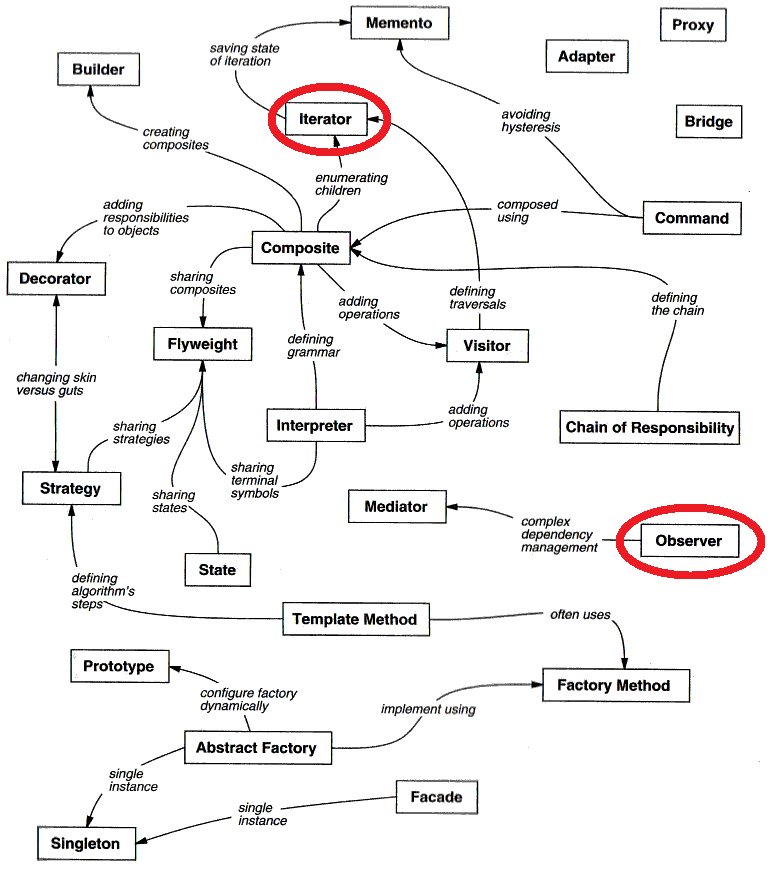
\includegraphics[width=0.48\textwidth]{figures/DesignPatternRelationships_bew.png}
	\end{center}
	\label{fig:designPatternRelationships}
	\caption{Relations between design patterns according to \cite{gamma1994-DesignPatternsGOF}}
\end{figure}

In 2010, Erik Meijer published a short paper called `\textit{Subject/Observer is Dual to Iterator}' \cite{meijer2010-Observable}, where he described a mathematical relationship between the Observer pattern and the Iterator pattern based on categorical duality. The paper shows that instances of the Observer pattern can be viewed as push-based collections, rather than the pull-based collections that result from the Iterator pattern. For later parts of this thesis, it is important to understand the mathematical basis of this relationship between the \obs and \obv interfaces in Rx and the \ieb and \ier interfaces in the Iterator pattern\footnote{For the purpose of the upcoming derivation we have chosen the C\# naming conventions of the Iterator pattern. In other programming languages these interfaces are respectively known as \code{Iterable} and \code{Iterator}.} (see \autoref{lst:itb-itr}).

In most common languages \ieb forms the basis of the Collections API. It has only one method \code{getEnumerator} that returns the \ier to iterate over the elements in the collection. The \ier interface on the other hand contains two methods to be implemented: \code{moveNext} and \code{current}. The former performs a side effect by moving a pointer to the next element in the iteration and then returns a \code{Boolean} to indicate whether or not there was a next element. The latter is a pure function that just returns the element the pointer is currently pointing to. Notice that the \code{moveNext} method can throw an exception rather than returning \code{false} in case an error occurs.

Besides providing these two methods, \ier in \autoref{lst:itb-itr} also extends the \id interface. This interface is meant to signal to the \ieb that no more elements will be pulled and that it can `start collaborating' with the garbage collector to clean up resources. The real meaning of \ier extending \id however, is that \code{getEnumerator} not only returns an \ier, but also returns something that is disposable. The \id interface is therefore not really part of \ier but rather a part of what \code{getEnumerator} returns \cite{E2E-Rx}. For now we will consider \id to be a silent bystander that is will be ignored in the derivation.

\begin{minipage}{\linewidth}
\begin{lstlisting}[style=ScalaStyle, caption={\ieb and \ier interfaces}, label={lst:itb-itr}]
trait IEnumerable[T] {
    def getEnumerator(): IEnumerator[T]
}
trait IEnumerator[T] extends IDisposable {
    def moveNext(): Boolean // throws Exception
    def current: T
}
trait IDisplosable {
    def dispose(): Unit
}
\end{lstlisting}
\end{minipage}

These two interfaces together form the basis of all pull-based or interactive collections as described in \autoref{sec:reactive-programming}. The user asks for the next element and will (eventually) get one in case a next element can be produced. In the following we will transform these interfaces for pull-based collections into interfaces for push-based or reactive collection, where the user subscribes to a collection and receives data once it is produced. This derivation, as well as its conclusion that interactive and reactive collections are each other's dual, is based on some categorical transformations and are discussed in several papers, as well as several keynotes and Channel9 video's \cite{meijer2010-Observable, meijer2012-YMIAD, E2E-Rx, meijer2014-Duality-And-The-End-Of-Reactive}. This derivation, as well as some of the intermediate steps are important for later parts of this thesis.

The first step in this derivation is to rewrite the two methods in the \ier interface into a single method \code{getNext()}. Using the categorical \textit{coproduct} \cite{rydeheard1988-Category-Theory} we can combine these two methods and determine its type signature: \code{getNext()} can either fail with an exception or succeed with either an element or no element, resulting in the type signature \code{getNext(): Try[Option[T]]}. The new, intermediate, set of interfaces is shown in \autoref{lst:itb-itr-interm}.

\begin{minipage}{\linewidth}
\begin{lstlisting}[style=ScalaStyle, caption={\ier interface after applying coproduct}, label={lst:itb-itr-interm}]
trait IEnumerable[T] {
    def getEnumerator(): IEnumerator[T]
}
trait IEnumerator[T] {
    def getNext(): Try[Option[T]]
}
\end{lstlisting}
\end{minipage}

Since both interfaces now only have one single method, and given that the only purpose of \ieb is to produce an \ier, they can be written as a single lambda expression. An \ieb can be written as:

\begin{equation} \label{eq:itb}
\code{() $\Rightarrow$ (() $\Rightarrow$ Try[Option[T]])}
\end{equation}

Notice that applying \code{Unit} to the outer lambda yields another lambda expression, which corresponds to the type signature of \code{getNext} in \autoref{lst:itb-itr-interm}: \code{() $\Rightarrow$ Try[Option[T]]}.

The next step in this transformation is to dualize \cite{rydeheard1988-Category-Theory} lambda~expression~\ref{eq:itb}. A very informal way of describing duality is to flip all the arrows and rewrite the lambda expression. For example, the duality of $f :: A \rightarrow B$ is $\bar{f} :: A \leftarrow B \equiv B \rightarrow A$. In the same way, we can apply this to lambda~expression~\ref{eq:itb}, resulting in

\begin{equation} \label{eq:obs}
\code{(Try[Option[T]] $\Rightarrow$ ()) $\Rightarrow$ ()}
\end{equation}

This lambda expression takes a lambda from \code{Try[Option[T]]} to \code{Unit}, and returns \code{Unit}.

We can now put this lambda expression back into context by splitting it into two interfaces. The inner lambda \code{Try[Option[T]] $\Rightarrow$ ()} can be rewritten to an interface called \obv, which has one method \code{onNext(t: Try[Option[T]]): Unit}. This method can then be further rewritten into three separate methods by expanding the \code{Try[Option[T]]} type: \code{onNext(t: T): Unit}, \code{onError(e: Throwable): Unit} and \code{onCompleted(): Unit}. The outer lambda on the other hand translates to an interface called \obs, which has one method \code{subscribe(obv: Observer[T]): Unit}. Notice how these interfaces are completely identical to the ones presented in \autoref{lst:obs-obv}.

%So far the presence of \id has been ignored in this derivation. This interface can however be found in \autoref{lst:obs-obv}, renamed as \subs. \todo{Add a couple of words on the functionality of \id and \subs and how they are the same.}

So far, the presence of \id has been ignored in this whole derivation. The reason for that is that this interface is considered to be a \emph{second} thing that is returned by the \ieb, rather than a supertype of \ier. What therefore basically happened in the derivation is that we only dualized the enumerator\textit{ness} and left the disposable\textit{ness} out of the dualization process \cite{E2E-Rx}. Therefore the dualized \ier, now called \obv, still extends from \id, even though this only means that we pass \textit{two} arguments to the \code{Observable.subscribe(obv: Observer)}. Just as the \id was meant to signal to the \ieb that no more elements will be polled and that it can clean up its resources, now \id signals to the \obs that it should stop sending data to the \obv. Finally, \id is renamed to \subs and its method \code{dispose} is split into two methods \code{unsubscribe} and \code{isUnsubscribed}.

% really dualized the enumeratorNESS but not the disposableNESS
% \ieb returned \ier AND \id
% now we dualized the enumeratorNESS, \id remained, so we need to return \id in \obs instead of void
% so when we subscribe to an \obs with an \obv, we get back a \id to unsubscribe later

This derivation shows that interactive, pull-based collections are the mathematical dual of reactive, push-based collections. The \obs and \obv interfaces can directly be derived from the \ieb and \ier interfaces. Both sets of interfaces can therefore be considered to be collections. In other words: streaming data behaves exactly the same way as regular collections, such as arrays, lists and sets, except for them being push-based rather than pull-based \cite{meijer2012-YMIAD, meijer2010-Observable}. In the world of push-based collections one \emph{subscribes} to the stream in order to \emph{react} to the next element that is being send, whereas one \emph{asks} for the next element in a pull-based scenario.

\subsection{\obs as a monad}
\label{subsec:obs-monad}
As described in the previous section, \obs can also be written as lambda~expression~\ref{eq:obs}. A better look at this expression reveals that \obs is actually a special instance of the \textit{continuation monad}, which has the following type:

\begin{equation} \label{eq:cont}
\code{(S $\Rightarrow$ R) $\Rightarrow$ R}
\end{equation}

In the \obs lambda expression, \code{S} is equal to \code{Try[Option[T]]} and \code{R} is equal to \code{()} or \code{Unit}.

Given that \obs is just a special instance of the continuation monad, it automatically has the two operators that are defined on all monads:

\begin{minipage}{\linewidth}
\begin{lstlisting}[style=HaskellStyle, caption={\obs as monad}, label={lst:obs-monad}]
newtype Observable t = Obs { runObs :: (t -> ()) -> () }

instance Monad Observable where 
    return :: Try[Option[T]] -> Observable[T]
    return t = Obs (\c -> c t )

    (>>=) :: Observable[T] -> (Try[Option[T]] -> Observable[S]) -> Observable[S]
    (Obs f) >>= g = Obs (\c -> f (\a -> let (Obs b) = g a in b c))
\end{lstlisting}
\end{minipage}

In the Rx implementation, these operators are present as well. The \code{return} creates an \obs from a \code{Try[Option[T]]}, meaning that it accepts either an error, or an empty value, or a non-empty value. Therefore \code{return} is split into three operators \code{apply(t: T)}, \code{error(e: Throwable)} and \code{empty()}. Since an \obs can have multiple values, \code{apply} is overloaded to have more than one value. This overload was already shown in section~\ref{subsec:core-comps} The \code{(>>=)} operator is renamed to \code{flatMap} and also splits the \code{Try[Option[T]]} parameter into three separate parameters \cite{rx-api}. Besides that, since the \code{T $\Rightarrow$ Observable[S]} parameter is used most frequently, the \code{flatMap} operator is overloaded with only this parameter.

A simple example of using these monadic operators in Rx is shown in \autoref{lst:monad-in-rx}. On line~\ref{line:return} the overloaded \code{apply} is called, which lifts four values into the \obs. The \code{flatMap} operator on line~\ref{line:flatMap} doubles the number of elements by creating an \obs that emits the value as well as the square of the value.

\begin{minipage}{\linewidth}
\begin{lstlisting}[style=ScalaStyle, caption={Monad operators in Rx}, label={lst:monad-in-rx}]
Observable(1, 2, 3, 4) |\label{line:return}|
    .flatMap(x $\Rightarrow$ Observable(x, x * x)) |\label{line:flatMap}|
    .subscribe(x $\Rightarrow$ print(x + " "))

// result: 1 1 2 4 3 9 4 16
\end{lstlisting}
\end{minipage}

\subsection{Operators}
\label{subsec:operators}
In section~\ref{subsec:derivation} we concluded that both the Iterator pattern and the Observer pattern are collections, only separated by the difference between push-based and pull-based behavior. All other rules on collections do however apply to both of them. In regular pull-based collections many operators are defined to manipulate, transform, filter, fold or group elements. These operators can therefore also be applied to push-based collections. One of them, \code{flatMap} was already shown in the previous section. However, rather than iterating over the pull-based collection and applying a transformation to each element, these operators \emph{react} to data being emitted by applying their particular transformation or side effect and passing the (transformed) data down to either a potential next operator or the \code{subscribe} method.

The Rx implementations of the \obs interface provide a wide variety of operators that apply all sorts of transformations to a data stream \cite{rx-api}. All operators are defined on \obs and will also return an \obs, making the API highly compositional. In order to understand how these operators work, we will look at some basic examples. Other, more advanced operators will be discussed in section~\ref{subsec:avoiding-overproduction}.

\paragraph{Filter}To select only those elements that satisfy a certain predicate, the operator \code{filter(p: T $\Rightarrow$ Boolean): Observable[T]} is used. Every time an element is received by this operator, the predicate \code{p} will be applied. If the element satisfies the predicate, it is passed downstream; otherwise the element will be discarded. \autoref{lst:operators-obs} shows in line~\ref{line:filter} how to select the odd numbers in a stream of integers by supplying a predicate.

\paragraph{Map}To transform one stream of data into another, the \code{map(f: T $\Rightarrow$ S): Observable[S]} is used. Each time an element (which is of type \code{T}) is received by this operator, the function \code{f} is applied to this element, yielding a new element of type \code{S}. This new element is then passed to down the stream. In \autoref{lst:operators-obs} the \code{map} operator is first applied in line~\ref{line:map} to the stream of filtered elements with a function that doubles the input.

\paragraph{Scan}Most operators do not allow for any form of internal state. They do not keep track of previous elements. An operator that can take the previous elements into account is \code{scan(seed: S)(acc: (S, T) => S): Observable[S]}. To this operator first of all a seed is supplied, which is the internal state of the operator before any value is received. Once an element is received, it will apply its internal state, together with that element to the accumulator function \code{acc} and produce an element to be emitted. This emitted value is also the new internal state of the operator. \autoref{lst:operators-obs} has a \code{scan} operator in line~\ref{line:scan} that takes the sum of all integers it receives and uses a \code{seed = 0}.

\paragraph{Drop}The \code{scan} operator is often used together with \code{drop(n: Int): Observable[T]}, which discards the first \code{n} elements and forwards all elements after that. The combination with the \code{scan} operator is used to prevent the seed value from being emitted further downstream, as is shown in \autoref{lst:operators-obs} line~\ref{line:drop}.

\paragraph{Take}Whereas \code{drop} discards the first \code{n} elements, \code{take(n: Int): Observable[T]} is used to only propagate the first \code{n} elements and discard all elements that come after that. In practice this means that the stream is terminated early with a call to \code{Observer.onCompleted()}. \autoref{lst:operators-obs} shows how \code{take} is used to only propagate the first and the second element and discard the third.

\begin{minipage}{\linewidth}
\begin{lstlisting}[style=ScalaStyle, caption={Operators on \obs}, label={lst:operators-obs}, columns=fixed]
Observable(1, 2, 3, 4, 5)		// emits:    1, 2, 3, 4,  5
    .filter(x $\Rightarrow$ x $\%$ 2 $==$ 1)			// emits:    1,    3,     5 |\label{line:filter}|
    .map(x $\Rightarrow$ x * 2)			// emits:    2,    6,    10 |\label{line:map}|
    .scan(0)((sum, x) => sum + x)	// emits: 0, 2,    8,    18 |\label{line:scan}|
    .drop(1)				// emits:    2,    8,    18 |\label{line:drop}|
    .take(2)				// emits:    2,    8 |\label{line:take}|
    .subscribe(x $\Rightarrow$ println(x))
\end{lstlisting}
\end{minipage}

Just as the interactive collections, Rx has defined its operators in a way that composition of operators is very easy. In this way, simple operators can be chained in order to create the complex behavior that is often desired. There are many more operators defined on \obs, which are not mentioned in this section. For a full overview, we refer to the documentation on the Rx websites \cite{ReactiveX, rx-api, Rx.Net}.

\subsection{Different kinds of streams}
\label{subsec:stream-kinds}
There are many kinds of observable streams that can all be implemented using Rx. For example, a clock or a timer is basically a stream of `ticks' that emits an element every time unit and therefore has a constant speed. A stream of keyboard events on the other hand emits an element every time a key is pressed and therefore most likely has a very irregular speed. A data stream can also be the result of a database query or a network call. In these instances it might take a certain amount of time before the first result is emitted, but every other result is received almost immediately after the first result appeared.

%\subsubsection*{Finite vs. infinite}
Some of these data streams, like the database query, are finite and will at a certain time in the future call \code{onCompleted}. Others, like the clock, will keep producing next elements forever, be it at a regular pace or quite irregular, like the keyboard. This kind of stream will never call \code{onCompleted}, but still may terminate with an error by calling \code{onError}.

%There exist many operators in Rx to control these particular cases. Infinite streams can be limited by using operators like \code{take(n: Int)} (see section~\ref{subsec:operators}), \code{takeUntil(predicate: T $\Rightarrow$ Boolean)} and \code{takeWhile(predicate: T $\Rightarrow$ Boolean)} that propagate all elements until or while a certain predicate is satisfied. Streams that terminate with an error can be resumed by operators like \code{retry()} or \code{onErrorResumeNext(resume: Throwable $\Rightarrow$ Observable[T])}, which respectively resubscribe to the same \obs or subscribe to another \obs.

%\subsubsection*{Hot vs. cold}
One other difference between certain streams is what happens when one subscribes multiple times to the same stream. Clocks or keyboard events, like broadcasters, emit values whether or not anyone is subscribed. If no one is subscribed, the events are still produced, but are immediately discarded. On the other hand, if multiple observers subscribe to the same stream, they will all receive the same events. This kind of stream is referred to as a \textit{hot} stream.

Some streams, like the \code{Observable(1, 2, 3, 4)} in section~\ref{subsec:core-comps}~and~\ref{subsec:obs-monad} or the database query, are not considered to be broadcasters. This kind of stream will create a new instance of itself every time an \obv subscribes to it. A second subscriber therefore receives the same result as a first subscriber, even though the second subscribes much later than the first one. This kind of stream is referred to as a \textit{cold} stream.

%A hot stream can be converted to a cold stream by sharing a single subscription with all observers. This can be done by operators like \code{share()} and \code{publish(f: Observable[T] $\Rightarrow$ Observable[S])}.

Notice that even though these differences do exist, they are not reflected in they type of the \obs. It is therefore always good to be careful with these distinctions and not to make any assumptions on streams being hot, cold, finite, infinite or error prone.

\subsection{Subjects}
A \subj can be viewed as a bridge between the \obv and the \obs. It can be subscribed to like an \obs, but can also observe another stream like an \obv. This is a very powerful tool that is often used as a starting point for a stream. Every time a certain event happens outside the context of the \subj, its \obv part can be called using the three methods. It will then process these events in its \obs part and propagate them down the stream.

A \subj can also be used to convert a cold stream into a hot stream. For this, a cold \obs is subscribed to the \subj. Because of this subscription, the cold \obs will be triggered to start emitting its events. The observable part of the \subj then becomes a hot \obs.

A special instance of \subj is the \bsubj, which behaves like a normal \subj but additionally emits its most recent value (or a seed or default value if none has been emitted yet) immediately after an \obv is subscribed to it. This is often used in user interface components like a text field to signal a certain initial state.

\section{Fast producers, slow consumers}
In the previous section we discussed that a reactive collection is equivalent to any interactive collection: it obeys the same rules and the same operators (like \code{map} and \code{filter}) can be defined. One difference however is that a reactive collection is push-based, whereas an interactive collection is pull-based. Rather than the consumer being in charge, asking for the next value, here the producer is in charge and \emph{it} decides when to emit a next value. The consumer just has to listen and can only react to the elements emitted by the producer. This is conform the definition of a reactive collection in section~\ref{sec:reactive-programming}: ``\textit{Reactive programs maintain a continuous interaction with their environment, but at a speed which is determined by the environment, not by the program itself.}''.

A risk that arises from allowing the producer to be in charge occurs when the consumer cannot keep up with the rate in which the producer is producing the data. This gives rise to the problem of what to do with the growing accumulation of unconsumed data.

A classic example of overproducing observables is the \code{zip} operator, which merges two (or more) streams by using a combiner function whenever both streams have produced an element. In this operator the problem occurs when one \obs always produces faster than the other. This is a problem, because \code{zip} cannot keep up with the rate in which the first \obs is producing, since the second \obs is much slower. The most common, but also slightly naive, implementation for this operator maintains an ever expending buffer of elements emitted by the first \obs to eventually combine them with the data emitted by the slower stream.

Ever expanding buffers is common answer to overproducing observables. A fast emitting stream is draining its data into a buffer and the much slower \obv eventually takes the data out of the buffer. The major problem with this solution (and thus with the implementation of \code{zip} as described above) is that the buffer will have to use an unwieldy amount of system resources.

\subsection{Avoiding overproduction}
\label{subsec:avoiding-congestion}
One way of dealing with overproducing observables is to simply avoid the problem and take proactive measures whenever it is expected happen. In the following we will discuss several ways to reduce the amount of data by using standard operators that are defined on the \obs interface. For this we distinguish two types of operators: lossy and lossless operators \cite{Backpressure-Explained}.

\subsubsection{Lossy operators}
One set of operators avoids the problem in a lossy way, meaning that some of the emitted data will be dropped.

\paragraph{Throttling} The \code{throttle(interval: Duration)} operator only propagates the first element that is received in a particular interval. All other elements are discarded. Once has finished, a new interval starts immediately, in which again the first received element is propagated and all other elements are discarded.

\paragraph{Sample} Rather than propagating the first element and discarding all others, the \code{sample(interval: Duration)} operator is used to discard all elements except for the last one that is received in a certain \code{interval}. This operator can for example be used when someone only wants to receive the data from a stock ticker every 5 seconds, without the need to process every value that comes in between.

\paragraph{Debounce} The operator \code{debounce(timespan: Duration)} will only propagate its received values after a certain \code{timespan} has passed without receiving an other value. When a value is received within the \code{timespan}, the previous value is discarded and the same process starts all over again with the newly received value. This operator is most commonly used in text fields within user interfaces, in order to avoid too much keystroke events being generated by a fast typing user. Rather than every keystroke being emitted, this operator will only yield the last keystroke after a particular \code{timespan}. Notice that in some versions of Rx this operator is also referred to as \code{throttleWithTimeout}.

With these operators many situations of potentially overproducing observables can be avoided by eliminating all the elements that do not really matter for a particular application.

\subsubsection{Loss-less operators}
Even though these lossy operators solve a large part of the problem, there are still as many cases left in which \emph{all} data that is send over a stream needs to be processed. For these kinds of use cases Rx provides so-called loss-less operators. These operators can buffer or group the data and emit collections of data, such that there are at least less elements to deal with.

\paragraph{Buffer} The \code{buffer} operator comes in a couple of different overloads. First of all, the \code{buffer(n: Int): Observable[List[T]]} operator, which receives data and groups it into lists of \code{n} elements. Once a list is filled (its size is \code{n}), it is emitted to downstream. Until then, the operator holds the data it receives. The \code{buffer} operator also comes in another form: \code{buffer(interval: Duration)}, which groups the data it receives within a certain interval into a single list. Finally there is \code{buffer[B](boundary: Observable[B])}, which groups the data it receives between two emissions of \code{boundary} into a single list.

\paragraph{Window} The drawback of a buffer is that it only propagates its received values once the buffer is filled, the boundary \obs fires or the interval is over. All the time in between no elements will be received by the observer or downstream operators. This already becomes clear from the return type: \code{Observable[List[T]]}. In order to accomplish the same behavior but with an \obs rather than a \code{List}, the \code{window} operator is included in Rx, having the same overloads as \code{buffer}. Instead of the list being emitted only once it is completely filled, the inner \obs is emitted as soon as the first element is received and is \emph{completed} once the size, interval or boundary requirement is met.

These operators form a first line of defense against overproduction. For streams where not all elements necessarily need to be processed (for instance the keyboard events on a text field), a lossy operator can be used. For streams where all emitted data is needed, a loss-less operator is the right solution. Besides that, for special occasions lossy and loss-less backpressure operators can be combined in order to create the optimal buffering strategy. This was discussed in some further detail in a conference talk at QCon by Ben Christensen \cite{christensen2014-RxServiceArchitecture}.

\subsection{Callstack blocking}
Another way of dealing with this problem is to block the callstack and with that `park' the thread on which the \obs is running. This directly slows down the producer and gives the consumer more time to process each element of the stream. Despite the fact that this approach goes against the `reactive' and `non-blocking' model of Rx, it can potentially be a viable option if the overproducing \obs runs on a thread that can safely be blocked.

This technique is currently not used in RxJava, but \emph{is} used in a particular implementation of the \code{zip} operator in RxMobile \cite{RxMobile}. Once either one of the streams emits a value, it is blocked until the other \obs has produced a value as well. In order to avoid blocking the upstream callstack completely, it is strongly recommended to switch each \obs to another thread or scheduler using the \code{observeOn} operator. With this only the callstack is blocked upto the start of this new thread or scheduler. Once the other stream has produced a value, the blocking of the first \obs sequence is removed and the \code{zip} operator waits until either one of the sources emits a next value.

\subsection{Reactive Streams}
Reactive Streams is an initiative \cite{Reactive-Streams} of a number of companies such as Netflix, Pivotal and Typesafe with the mission to \textit{provide a standard for asynchronous stream processing with non-blocking backpressure}. This collaboration resulted in an alternative API \cite{Reactive-Streams-API} for stream processing that is claimed to be capable of handling overproducing observables using backpressure.

This Reactive Streams API (see \autoref{lst:pub-sub}) looks fairly similar at first glance to the original API that was developed by Microsoft, but has some particular differences that have significant influence on the handling of backpressure. The \obs, renamed \code{Publisher}, looks the same: it still is parameterized over \code{T} and still has a \code{subscribe} method. The \obv, which was passed to the \code{subscribe} method, is replaced with a \code{Subscriber}, even though it is almost the same\footnote{The \code{onComplete} method in \autoref{lst:pub-sub} does not contain a typing error compared to \autoref{lst:obs-obv}. This is actually how the API is specified!}. It only adds an extra method \code{onSubscribe}, which is called right after the \code{Subscriber} is subscribed to the \code{Publisher}. This \code{onSubscribe} method requires an argument of type \code{Subscription}. This last interface contains two methods: \code{cancel}, which is similar to the \code{unsubscribe} method in \autoref{lst:obs-obv} and a new method \code{request(n: Long)}.

\begin{minipage}{\linewidth}
\begin{lstlisting}[style=ScalaStyle, caption={Publisher, Subscriber and Subscription}, label={lst:pub-sub}]
trait Publisher[T] {
    def subscribe(s: Subscriber[T]): Unit
}

trait Subscriber[T] {
    def onNext(t: T): Unit
    def onError(e: Throwable): Unit
    def onComplete(): Unit
    def onSubscribe(s: Subscription): Unit
}

trait Subscription {
    def cancel(): void
    def request(n: Long): Unit
}
\end{lstlisting}
\end{minipage}

This last method reveals the whole idea behind the Reactive Streams API, namely to let the \code{Subscriber} request a certain amount of elements from the \code{Publisher}. This way the \code{Subscriber} is in charge of how many elements it will receive eventually and the \code{Publisher} just has to send at most this amount of elements by calling the \code{onNext} method.

Taking a step back and evaluating the true meaning of what the Reactive Streams collaboration has come up with, results in the conclusion that this API is interactive rather than reactive, since it lets the consumer (\code{Subscriber}) be in charge of the rate at which data is sent to him. This is discussed in more detail in a conference talk at Lambda Jam 2014 by Erik Meijer \cite{meijer2014-Derivation}. Compared to the earlier discussed \ieb collections, it only adds the features of non-blocking and requesting more than one element (which is what the \ieb interface technically does) per request. We will discuss the consequences of this API in more detail in a later section.

\subsection{Reactive pull}
The ideas that sprout from the Reactive Streams initiative have been incorporated in the RxJava library. They kept the original naming conventions of \obs and \obv but added a couple of new methods to the latter: \code{request(n: Int)}, which signals to the \obs that it will be able to handle \code{n} new elements and \code{onStart()}, which performs the initial request from the \obv to the \obs. After the initial request is done, the \obs sends at most \code{n} elements to the \obv, which receives them in the \code{onNext} method. This is now the place where the \obv can call \code{request} again to receive more data.

We recognize these two methods from the Reactive Streams API, where \code{onStart()} was called \code{onSubscribe} and \code{request(n: Long)} was inside the \code{Subscription} interface. Making these slight modifications does not change the intention of the Reactive Streams API: it introduces a feature called \textit{reactive pull} in the \obv to manage the number of elements that are emitted by the upstream \obs.

Earlier versions of RxJava, who did not have this feature only had the ability to communicate upstream by calling the \code{unsubscribe} method. Recall that when an unsubscribe occurs, the \obs is basically signaled to stop emitting any data to the \obv. Besides unsubscribing there was no way in the standard Rx model to communicate upstream.

This feature from Reactive Streams allows the \obv to have some more control by \emph{pulling} from the data source (\obs) at its own pace. RxJava is set up in such a way that processing data under normal circumstances is still push based. Only when the \obv can't handle the speed in which data is sent, it will switch to this pull based model. Wrapping it up in this way, the problem of overproduction is not prevented or gone away but is rather moved up the chain of operators to a point where it can be handled better \cite{RxJava-Wiki-Backpressure}.

With this it limits the number of elements that are in a buffer within certain operators. Using this new feature, the earlier mentioned \code{zip} operator is implemented by using a small buffer for each \obs. It only requests items from one of these sources when there is room for more elements in its buffer. Once all buffers contain at least one element, the operator can remove an element from each buffer, zip these together and push them downstream. After that there is room for at least one extra element in all buffers, hence new requests are sent to the upstream.

Notice that the RxJava wiki \cite{RxJava-Wiki-Backpressure} points out that this method only works when all streams that are zipped together respond correctly to the \code{request()} method. This is \emph{not} a requirement for the normal \obs, but it is required for instances of \obs that are used in operators like \code{zip} that depend on reactive pull. RxJava therefore provides operators such as \code{onBackpressureBuffer} and \code{onBackpressureDrop} that respectively buffer and drop data that cannot be consumed immediately by the downstream \obv.

\subsection{Transmission Control Protocol}
A well known protocol from the Internet protocol suite is the Transmission Control Protocol (TCP), which offers reliable delivery of streams of data between applications communicating over an IP network \cite{tanenbaum2011-Computer-Networks}. In order to avoid having a sender to send data too fast for the TCP receiver to receive and process the data, it uses an end-to-end flow control protocol with a sliding window. The receiver specifies in the TCP header's \textit{Window Size} what amount of additional data it is willing to receive and buffer for the current connection. The sending host can only send at most that amount of data and has to wait for an acknowledgment and window update from the receiving host.

In case the sender receives a window size of 0, it obviously cannot send any data and instead starts a so called \textit{persist timer} that protects the TCP connection from a permanent deadlock. When this timer expires without the sender having received any new window sizes, it will send a small packet in order of the receiver to send a new acknowledgment containing a new window size.

The problem solved by this flow control protocol is in fact the same as overproducing observables discussed in this section. The solution presented by TCP is similar to \textit{reactive pull} and \textit{Reactive Streams} in the sense that they too advertise an `available buffer space message' to the \code{Producer} or \obs by calling the \code{request} method. The difference with TCP is that the earlier discussed solutions do not have the need for a persist timer since deadlock from lost window updates is not possible.

\todo{something more on this???}












































\clearpage
\chapter{Controlling overproduction}
\label{chap:exploring-the-problem-space}
In the previous chapter we established the definition of a \textit{reactive program} in terms of its behavior, how it is implemented in Rx, what the danger is of having an overproducing \obs and which solutions already exist to solve this problem. In this chapter we will discuss these solutions in further detail, consider their advantages and disadvantages and argue which solutions work for the various kinds of streams.

\section{Hot and cold streams}
Applying the definition of reactiveness by Benveniste and Berry \cite{berry1991-Reactive} to the Rx \obs, we can conclude that every \obs sequence starts with a source that emits values at its own pace. No matter which function is used for this (\code{apply}, \code{range}, \code{timer}, \code{interval}, etc.), ultimately they all are the result of the \code{Observable.create} function. This function lifts an arbitrary source into the \obs interface and treats its values like streaming data. The behavior that is exposed by the resulting stream can however differ from source to source.

Sources like clocks, mouse moves or key presses start emitting whenever it desires, regardless of any \obv being subscribed to the stream. When no one is listening, the data is simply discarded; when multiple \obv instances are subscribed, every one of them receives the same data at (approximately) the same time. In case an \obv subscribes on a later moment, it will not receive all previously emitted data, but will only share in the data that is send after it is subscribed. This kind of source is considered to be \textit{hot}. It is strictly reactive, meaning that it can only emit data at a speed which is determined by the source and has no way to be slowed down by any \obv that cannot cope with the amount of data sent.

On the other hand there are streams that originate from sources that are actually interactive. These include the results of database queries and \ieb sequences. Often the reason for them being wrapped into an \obs is because of a potential delay that needs to be awaited before the result is returned, without blocking the program flow or call stack. It may, for example in case of lazy evaluation, take some time before the \ier has produced its next element. The \obs will however not start emitting its data immediately, like the hot variant, but will wait until at least one \obv is subscribed. Only then it will start producing its values. In case a second \obv subscribes, the stream will effectively duplicate itself and start all over again with emitting the first values. Unless specified by operator sequences, this means that the lazy \ier in the source will have to produce its values a second time as well. In the end, both the first and second \obv have received the same set of data, even though the second subscribed much later than the first. A stream with this kind of behavior is referred to as a \textit{cold} \obs.

In the rest of this chapter we will distinguish between two types of the cold \obs. First there is the \textit{cold with-latency \obs}, which is bound by a certain notion of time. This type wraps a source that is interactive, but can take some time before it produces its next element. Examples of this can be a network response, the result of a database query or an \ieb sequence where each element is computed lazily and therefore takes some time to be returned. On the other hand we distinguish the \textit{cold no-latency \obs}, which is \emph{not} bound to any notion of time. This type mainly wraps interactive sources for which the values are already computed, such as a list.

In short, a hot \obs has a source that is strictly reactive, whereas a cold \obs originates from a source that is interactive. With the latter, an \obv could potentially ask the \obs to slow down by generating elements less frequently, even though this would strictly speaking be against the definition of reactiveness. The \obs would not have to buffer unbounded amounts of elements that cannot be consumed immediately, it will just generate its elements in a slower pace.

This is however not possible for a hot \obs, since it reacts to events from the outside environment. It is not possible for an \obv to ask the source to slow down the movement of the mouse, nor is it possible for the \obv to request less frequent key presses or clock ticks. These events are dependent on a notion of time; their speed is determined by the environment \cite{berry1991-Reactive}.


\section{Solutions for overproducing sources discussed}
In the previous chapter we described an interesting problem that occurs when working with streaming data and reactive programming: ``\textit{what happens when the consumer cannot handle the data flow presented by the producer?}''. We also presented a number of solutions, ranging from putting data in an overflow buffer to gaining more control over the \obs. Some of these solutions work perfect under certain conditions, others do not. In this section we will discuss the solutions that were described in section~\ref{sec:fastproc-slowcons} in further detail and reflect on them in the light of the previous section on hot and cold streams.

\subsection{Avoiding overproduction}
As described in section~\ref{subsec:avoiding-overproduction}, \textit{avoiding} is a first line of defense for overproduction. This was done by introducing several operators that either drop some of the data or buffer the data and propagating these buffers downstream for further manipulation. All lossy operators, as well as the \code{buffer} with interval, require a \sch for them to run their interval timers on, hence the output stream of these operators runs on a different thread.

For a hot \obs this kind of defense mechanism is perfect, as the speed at which the source is producing is unknown. This also holds for the cold with-latency \obs, as the production of elements is also bound to a notion of time. For other cold streams, like \code{Observable(1, 2, 3, 4)} or an \obs that is created from a list of elements as shown in \autoref{lst:obs-from-seq}, it does not make any sense to add any overproduction-avoiding operators, as this kind of stream is sequential and will in fact emit at a rate which is determined by the \obv.

\begin{minipage}{\linewidth}
\begin{lstlisting}[style=ScalaStyle, caption={Observable from \code{Seq[T]}}, label={lst:obs-from-seq}]
def fromSeq[T](list: Seq[T]): Observable[T] $=$ {
    Observable.create(observer $\Rightarrow$ {
        list.foreach(observer.onNext)
        observer.onCompleted()
    })
}
\end{lstlisting}
\end{minipage}

We are aware of the fact that these operators also have use cases other than avoiding overproduction, such as edge detection or calculating the derivative of a stream of numbers. However, these use cases fall outside the scope of this thesis and for them the comments above do not apply.

\subsection{Callstack blocking}
Subscribing to an \obs is basically nothing more than supplying an \obv to the function within \code{Observable.create} and \emph{sequentially} executing this function using this provided \obv. Once an element is emitted by the source, all operations in the \obs sequence are executed on that element before a second element is emitted. In the sequence of operators in \autoref{lst:operators-obs}, first all operations on $1$ are performed, before $2$ is emitted by the \obs (and then discarded by \code{filter}). This is also the case in \autoref{lst:observeOn} up to line~\ref{line:observeOn-in-observeOn}, after which the elements are scheduled on a different thread and hence are further processed in parallel with emitting new elements from the source.

The order of operations is designed this way to allow for lazy evaluation: never run code that does not need to be run. If a cold \obs contains 5 elements and the operator sequence contains the operator \code{take(2)} (see \autoref{lst:lazy}), only the first 2 elements from this \obs will be evaluated, rather than all 5. After the second element has passed \code{take}, it sends an \code{onCompleted()} downstream, right after the second \code{onNext}, causing the stream to end without evaluating the other 3 elements.

\begin{minipage}{\linewidth}
\begin{lstlisting}[style=ScalaStyle, caption={Lazy evaluation}, label={lst:lazy}]
Observable(1, 2, 3, 4, 5)
    // some operators
    .take(2)
    // some more operators
    .subscribe(i $\Rightarrow$ print(i + " ")) // only prints the first and second element
\end{lstlisting}
\end{minipage}

Following this order of operations, we can conclude that basically every higher order function that is executed in the operator sequence is in a sense blocking the callstack during its computation and thereby preventing the source from emitting a next element until the previous element has gone through the whole operator sequence. This is the reason why we concluded in the previous section that avoiding overproduction on a cold no-latency stream does not make any sense. The rate of emission is already determined by the speed in which all operators together are executed.

This is also true for any other kind of stream, whether it is hot or cold, whether or not it has latency and no matter what kind of source emits these elements. This may seem quite surprising, especially for the hot \obs, since we always claimed that this operator is only controlled by its outside environment. However, an example of this is shown in \autoref{lst:blocking-hot-obs}. Here a cold \obs is subscribed to a \subj (line~\ref{line:blocking-hot-subject-subscribe}), making it hot, according to section~\ref{subsec:subjects}. At several points in the operator sequence the time passed since \code{start} is printed and on line~\ref{line:blocking-hot-sleep} the callstack is blocked for 1 second by pausing the thread this whole process runs on. The console output of executing \autoref{lst:blocking-hot-obs} is provided in \autoref{lst:console-output-blocking-hot}\footnote{Due to the inner workings of the JVM, the times shown here may vary by a couple of milliseconds from execution to execution.}.

\begin{minipage}{\linewidth}
\begin{lstlisting}[style=ScalaStyle, caption={Applying callstack blocking on a hot \obs}, label={lst:blocking-hot-obs}]
def now = System.currentTimeMillis()
val start = now
def timePassed = now - start

val timer = Observable(1, 2, 3, 4)
    .tee(i $\Rightarrow$ println("[" + timePassed + "] emitted - " + i))
val subject = Subject[Int]

subject.tee(i $\Rightarrow$ println("[" + timePassed + "] before - " + i))
    .tee(_ $\Rightarrow$ Thread.sleep(1000)) |\label{line:blocking-hot-sleep}|
    .subscribe(i $\Rightarrow$ println("[" + timePassed + "] after - " + i))
timer.subscribe(subject) |\label{line:blocking-hot-subject-subscribe}|
\end{lstlisting}
\end{minipage}

\begin{minipage}{\linewidth}
\begin{lstlisting}[style=ScalaStyle, caption={Console output from \autoref{lst:blocking-hot-obs}}, label={lst:console-output-blocking-hot}]
[47] emitted - 1
[47] before - 1
[1059] after - 1
[1059] emitted - 2
[1059] before - 2
[2060] after - 2
[2060] emitted - 3
[2060] before - 3
[3062] after - 3
[3062] emitted - 4
[3062] before - 4
[4064] after - 4
\end{lstlisting}
\end{minipage}

From these results it becomes clear the first value was emitted at $t=47\ ms$. Almost immediately after that, the thread on which the whole program is running is blocked for 1 second. At time $t=1059\ ms$ the first value is propagated to the \code{subscribe}. \emph{Only then} the second item is emitted by \code{Observable.apply}.

We can now conclude that even a hot \obs can be controlled by callstack blocking. Notice however that this creates a (potentially ever expanding) buffer of unprocessed \code{onNext} calls within the \code{Observable.create}'s callstack, using an excessive amount of memory. With that we only emulated the naive solution to overproducing streams (see section~\ref{sec:fastproc-slowcons}) by using callstack blocking. The same buffering behavior can also happen within the \code{observeOn} operator, when the other thread used callstack blocking to slow down the stream.

The case described above is one where the thread cannot be blocked safely. It can potentially blow up the program when the buffer gets too big. This is what RxJava warns against in its wiki\cite{RxJava-Wiki-Callstack-Blocking} and what RxMobile warns against in the context of the particular \code{zip} implementation discussed in section~\ref{subsec:callstack-blocking} \cite{RxMobile}. Only certain kinds of operators can use callstack blocking safely, provided with streams that can handle this callstack blocking safely.

Another issue with a hot \obs is what happens when more than one \obv is subscribed and both do callstack blocking. This can potentially lead to even more disastrous situations, where a fast \obv suffers from a slower one and where deadlock situations are inevitable.

In general we can conclude that controlling the flow of data by callstack blocking is already implicitly used in cold no-latency stream, but that it is no good to use callstack blocking on a hot or cold with-latency \obs, unless the developer is completely certain of the stream's behavior.

\subsection{Reactive Streams}
A third way of managing the overflow of data is by using the backpressure technique that was found by the Reactive Streams initiative. The associated API, discussed in section~\ref{subsec:reactive-streams}, consists of a \code{Publisher} that corresponds to the \obs, a \code{Subscriber} that adds an \code{onSubscribe} method to the \obv and a \code{Subscription} with a \code{cancel} and \code{request} method that replaces the Rx \subs. The intention of this API is to let the consumer be in charge rather than the producer. It is the consumer that dictates how many elements it wants to receive and with that it follows the design of the TCP protocol (see section~\ref{subsec:tcp}) as the receiver also sends window size updates (how much more data it is able to handle) to the sender.

The most important question to ask here is whether or not the approach of Reactive Streams is a solution to overproducing sources in reactive programming, as is advertised on the website and implied by the name \cite{Reactive-Streams}. To answer this question, we first need to reflect on the previous paragraph: the consumer is in charge and the producer can at most send the amount of data that is requested by the consumer. Following the definitions from Albert Benveniste and G\'erard Berry \cite{berry1991-Reactive} on reactive and interactive programs (see section~\ref{sec:reactive-programming}), we must conclude that this API creates an \emph{interactive} program, that ``\textit{interacts at its own speed with users or with other programs}'', in this case with the \code{Producer}.

Besides that, we need to take into consideration that `reactive' is the dual of `interactive'. In other words, the interactive interface needs to be dualized in order to become reactive. However, the Reactive Streams API can be constructed from \ieb without using any dualization techniques, as shown by Erik Meijer during a conference talk at Lambda Jam 2014 \cite{meijer2014-Derivation}. Instead he shows that techniques like coproduct, continuation passing style and currying will suffice. This too shows that the Reactive Streams API is not reactive at all, but is interactive instead.

Reactive Streams, even if it is interactive, rather than reactive, still distinguishes itself from the classical set of interactive programming interfaces: \ieb and \ier. Rather than calling \code{moveNext} and \code{current}, a \code{Subscriber} can advertise to its \code{Producer} that it can handle \code{n} more element. It is then up to the latter to send these elements either immediately or after some amount of delay to the former by calling the \code{onNext} method or signal the end of the stream by calling \code{onCompleted} or propagating an error by calling \code{onError}. Just as Rx, the API is set up in such a way that it does not block the program flow, which would be the case when using \ieb and \ier. In that sense, Reactive Streams is definitely not the same as \ieb and \ier, but is rather an API for \textit{asynchronous interactive programming}; it is not just a pull model, it is an \textit{asynchronous} pull model.

The question of whether Reactive Streams is able to solve the regulation of overproducing sources in reactive programming still remains. As we understand now what the API really is (an asynchronous pull model), we can finally reason about what kind of sources it can wrap and with that replace the Rx API.

Both a cold no-latency source and a cold with-latency source are perfect candidates to be wrapped in this kind of stream as they are already interactive by themselves. The \code{Subscriber} can pull as much data from the source as it wants, only restricted by the size of the source, in case it is finite. Note that for the no-latency source the response of a request will be immediate, whereas the with-latency source will take some amount of time to produce its next \code{n} values.

A hot source on the other hand is not as suitable for the Reactive Streams API as the cold sources are. There is no way for the \code{Producer} in which the hot source is wrapped to interact with it. It cannot request the next \code{n} elements from it, nor can it request to slow down or speed up. This is implied in the nature of a hot source. The only way to have a hot source be wrapped in a \code{Producer} is to drain its the data in a buffer or queue and sending the requested amount of elements from this buffer to the \code{Subscriber}. In general this is again that dangerous move of possibly storing unwieldy amounts of data for later processing as is described in earlier sections. That being said, in special cases, where in the long term the downstream can empty the buffer before it starts overflowing, it is in fact possible to use this API for it. An example of this may be a source with bursty behavior, where in a short amount of time a large amount of data is produced, after which no data is produced for a longer amount of time.

\subsection{RxJava and reactive pull}
RxJava started of as a port of Rx.Net for the JVM and was until version 0.20 purely reactive. It did not have any other policies for handling backpressure than the ones discussed in section~\ref{subsec:avoiding-overproduction}. In version 0.20 backpressure support was introduced as a result of collaborations with the Reactive Streams initiative. This implementation (also referred to as \textit{reactive pull}) did not change the original Rx interfaces but rather added extra methods that were taken from the Reactive Streams API. Due to these changes, the reactiveness is partially lost, as the data flow was now controlled by \code{request(n)} calls from the \obv.

From version 0.20 onward, RxJava has a lot of similarities with the Reactive Streams API in terms of handling backpressure. It is therefore well equipped to handle cold sources by wrapping them in the \obs. However, in contrast to Reactive Streams, this API is still able to correctly coop with hot sources. The RxJava wiki states that for this the \obs needs to be initialized with \code{request(Long.MAX\_VALUE)}, which orders the \obs to emit data at its own pace \cite{RxJava-Wiki-Backpressure}.



























%\section{Your mouse is NOT a database!}
\label{sec:your-mouse-is-not-a-database}
Looking through the architecture of Java's interactive collections API, one can immediately notice the amount of interfaces that inherit from \itb \cite{java-iterable-api}. Whilst this \itb only contains a getter for the \itr interface, the subinterfaces of \itb supply more functionality. For example, the \code{Collection} interface introduces functionality for adding, removing, querying and transforming a dataset. It however does not specify the exact behavior of these methods. This is done in more specialized subinterfaces of \code{Collection}. The \code{Set} interface has different behavior on adding an element than the \code{List} or \code{Queue} interfaces. And even within these interfaces the details vary per implementation. A data structure like \code{ArrayList} has the benefit of very efficient random access, but is slower in adding and removing elements in the list \cite{linkedlist-vs-arraylist}. The \code{LinkedList} on the other hand does way better on adding and removing but is not as efficient in doing random access. The \code{Set} interface has also various implementations that provide different behavior. Besides all of that, there is a whole other realm of collection interfaces, specialized in handling concurrency, that contain many more implementations but still all inherit from that same \itb interface.

This inheritance tree of Java's collection API was created the way it is because the authors saw that different circumstances required different data structures that on the one hand all shared the same concept of being able to be iterated over, but on the other hand differed in behavior from other points of view. Even though these data structures shared some commonalities, they had just as many differences in their behavior.

In languages like Scala a similar architecture is used. However, besides the \itb containing a getter for the \itr interface, it also provides and implements many higher-order functions that are able to manipulate the data structure, such as \code{map}, \code{filter}, \code{fold}, \code{reduce} and \code{flatMap}. Other interfaces and classes that inherit from Scala's \itb interface automatically inherit these functions and are expected to behave in such a way that these functions can operate correctly. The various implementations of \itb are allowed to reimplement these functions to make them run more efficient, but are not allowed to alter their behavior.

When we demonstrated the derivation of the \obs collection in \Cref{subsec:derivation}, we argued that, since we only dualized the \textit{interactiveness} of the \ieb to the \textit{reactiveness} of the \obs, all other rules on collections should still apply. This implies that the concept of higher order functions such as \code{map}, \code{flatMap} and \code{fold} on \ieb is still valid, even though these have to be reimplemented to conform to the reactiveness of the \obs collection. Notice that the result of using these functions is not allowed to be different from performing them on any \ieb collection! It is just the implementation that is changed due to the reactiveness.

In contrast to the many subinterfaces and implementations of \itb, a library like Rx, as discussed in \Cref{chap:problem-statement}, has shown only a single interface for (reactive) collections. However, in the previous sections of this chapter we have identified several classes of sources in the light of overflow protection that would greatly benefit from several implementations of the \obs interface. At this point the Rx interface is mainly specialized for hot sources, that do not allow for any form of interaction. Cold sources can be wrapped in this interface as well by simply not interacting with them and only iterating over them as if they had no possibility for interaction.

Even though cold sources do theoretically not belong in the world of a reactive interface, one could argue that these sources are more convenient to work with in the context of a reactive interface. First of all, the Rx interface provides a great way of handling and recovering from errors as well as dealing with completion events. If this had to be done with separate types, such as \code{Try} and \code{Option}, it would be too much of a pain to do so, as monads do not compose greatly. With Rx one can deal with \code{onError} and \code{onCompleted} events and continue continue composing operators after that. Secondly, the Rx interface provides much more operators than similar \itb based interfaces do, allowing for more complex programs to be written in a functional and compositional style. Also the option to schedule work on a different thread or thread pool is a nice addition to the API and removes a lot of boilerplate code (and associated bugs!) that deals with concurrency. Fourth, one can be forced into wrapping an interactive collection in a reactive interface due to the fact that the context (e.g. a constructor or method parameter) requires such an interface. Finally, one could argue that the reactive interface is much more intuitive in regards to the consumption of data and that it is more expressive to use \code{onNext}, \code{onError} and \code{onCompleted} in order to declare what the consumer needs to do with the data it receives.

In practice, one might want to wrap the \code{ResultSet} from a database call into an \obs and schedule it on a different thread in order to not block the applications main thread from the point of sending a query to the database and until the whole \code{ResultSet} is processed. With the query handling on a different thread, the application can for example still process mouse events on the main/ui thread by responding to these events. Notice that in both cases the \obs type is used, even though one \emph{can} pull from a \code{ResultSet} but \emph{cannot} pull from a mouse. Clearly your mouse is NOT a database and therefore they should be treated differently!

Just like the original interface for reactive programming is mostly optimized for wrapping around hot sources, one could imagine an interface for handling cold sources. One could subscribe to this interface, from which point onward this interface would pull data from the cold source on behalf of the subscriber. This would mean a segregation between the purely reactive interface and its implementation of the higher order functions and operators that are applicable to reactive sources on the one hand and the operators that are focused on interactive sources on the other hand.

One could also imagine the backpressure techniques that are currently provided and implemented by Reactive Streams and RxJava to be in this subinterface for interactive sources. This segregation would solve the issue with the Reactive Streams design of its disability to wrap around a reactive source. A drawback of this design, which we already discussed in the previous section, is the fact that a large portion of the operators and higher order function probably need to be reimplemented for this interface.

The segregation of these interfaces would most likely greatly benefit the performance of a library like RxJava. Currently when one uses the RxJava \obs to wrap around a reactive source, it still has to deal with all the backpressure support that is in a large portion of the operators. Some operators like \code{zip} currently even throw exceptions when backpressure support is not explicitly added, for example by operators such as \code{onBackpressureBuffer} and \code{onBackpressureDrop}. This is not a great way of working, as there is no way for the developer to have this issue checked at compile time. Preferably the need of a certain backpressure behavior should be indicated on the type level or at least be silently applied in a default behavior, without bothering the developer with it and causing errors at the unlikeliest of moments (a.k.a. production).

Besides performance, splitting the uses for RxJava's \obs interface into two or more interfaces would also greatly benefit the usability of the whole library. On the one hand, one could have the \textit{reactive} \obs interface, which is suitable for wrapping around hot sources\footnote{this is more or less what the library looked like before verison 0.20} and implements all operators without the use of backpressure. Then on the other hand the library could have the \textit{interactive} \obs interface, which is suitable for wrapping around cold sources. This interface would most likely inherit from the reactive \obs interface, as this interface already contains the contract of the producer being in control.

A third benefit of splitting RxJava's \obs interface is that with multiple interfaces a developer can be more expressive on the language's type level. Currently neither the developer nor the compiler can derive whether an \obs behaves like a cold or a hot stream based on the type of \obs. This would be greatly beneficial, especially in more complex operations for which in some cases operators like \code{publish(selector)} need to be used, whereas in other cases their use is redundant. The compiler and type system being able to determine whether or not these operators are available would also greatly improve the usability.

%\section{A new approach}
Splitting the \obs interface into a base interface that is focuses on hot sources and a subinterface that is optimized for cold asynchronous sources brings up the issue of how much to put in this subinterface. After all, the contract of the producer of the data being in charge and the consumer reacting to the received data is already in the base interface, just as the operators that gives Rx its great value of compositionality and its ability to do asynchronous computations.

One way to go is to implement backpressure in this subinterface as envisioned by Reactive Streams. This however would require an implementation like `post v.0.20' RxJava with the \code{Producer} interface added to to the architecture as well as a reimplementation of the operators that require backpressure support. Note that this implies that within the operator sequence the stream would be interactive rather than reactive. Also note that we already discussed some problems with this implementation in sections~\ref{subsec:handling-overproduction-with-reactive-streams}~and~\ref{subsec:handling-overproduction-with-rxjava}.

As pointed out by the RxJava wiki \cite{RxJava-Wiki-Backpressure}, backpressure does not make the problem of an overproducing source go away. It only moves the problem up the chain of operators to a point where it can be handled better. This means that a \code{request(n)} call from the \code{zip} operator in section~\ref{sec:fastproc-slowcons} goes up the chain to the point where it can fulfill that request. This is either an operator like \code{onBackpressureBuffer} or \code{onBackpressureDrop} or the source that is wrapped in an \code{Observable.create} or one of its higher abstractions.

Another way to go with the implementation of the subinterface is to decouple the flow control from the operators and move it to the origin of the stream. This way we can keep the API clean, we do not have to take this flow control into account while implementing new operators, we do not have to reimplement the operators inherited from the base interface and (most importantly) we can keep the operator sequences reactive.

For this approach we need to observe that the \obs is nothing more than just a source wrapped in \code{Observable.create}, from which this source instantly gains all the operators, the possibility to go asynchronous and to potentially be composed with other sources using operators such as \code{flatMap}, \code{combineLatest}, \code{withLatestFrom} and \code{zip}.

Instead of wrapping a cold source in the \code{Observable.create} as is currently done in RxJava, we propose to wrap it in a universal interactive interface (such that communication with the source is not coupled with its own specific interface) and let a function equivalent to to \code{Observable.create} pull the data out of the source via this interface on behalf of the one who subscribes. The data is then put into a bounded buffer, from which it is pulled again by a downstream \obs that operates on a different thread. Once an element is pulled from the buffer, it will block the downstream \obs's callstack from pulling another element until the current element is fully processed or taken over by a third thread. In the mean time the buffer can request new elements from the source and by doing so keeps the downstream \obs as busy as it possibly can without letting it wait for a new element to be produced by the source.

\begin{figure}[H]
	\begin{center}
		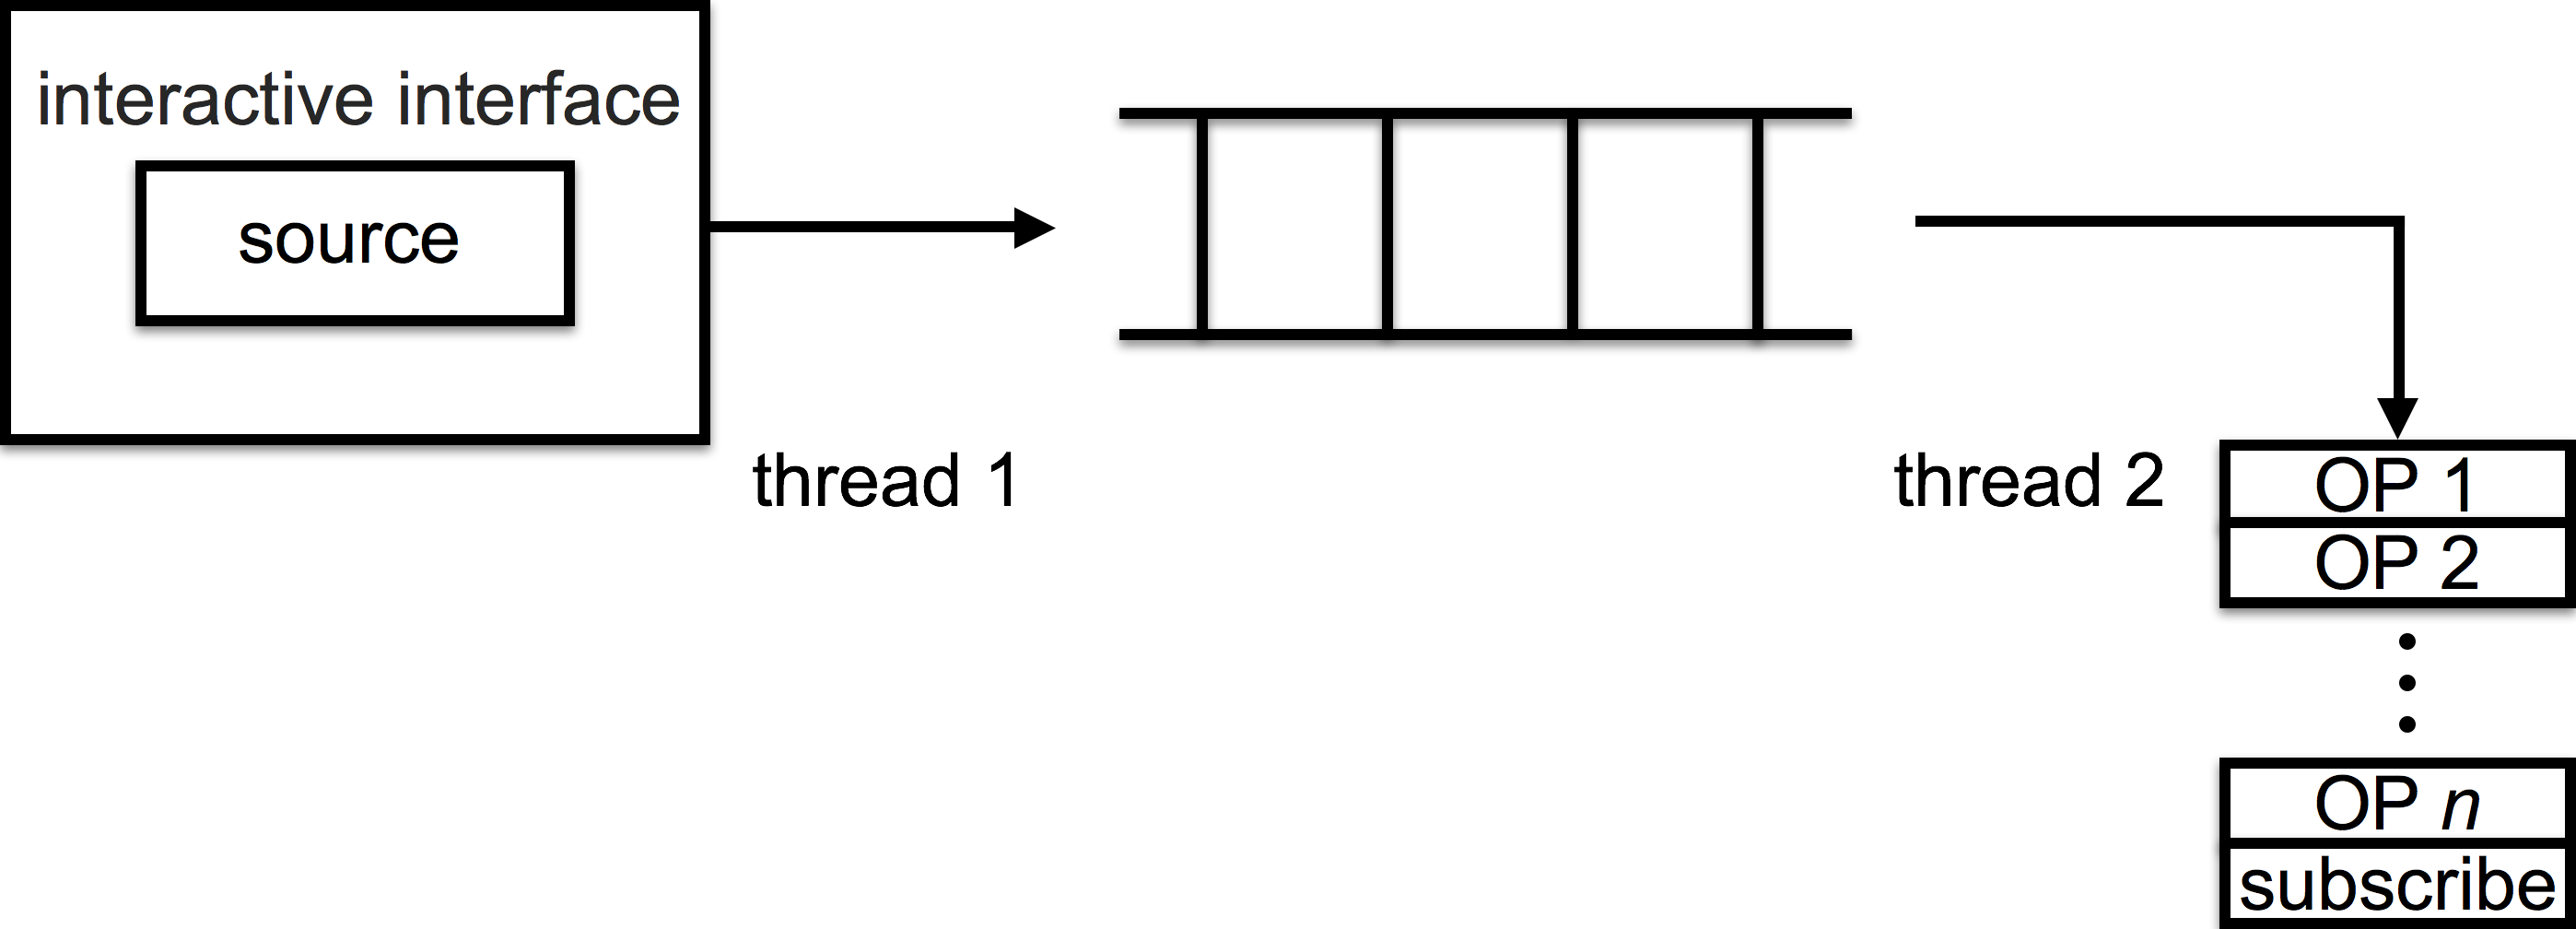
\includegraphics[width=0.63\textwidth]{figures/Approach.png}
	\end{center}
	\caption{Schematic representation of our approach}
	\label{fig:new-approach}
\end{figure}

With this approach we have reduced the problem of overproduction to a problem of controlling the size of a buffer to be as small as possible, without the buffer being exhausted by a fast consuming downstream. A buffer size that is too small can lead to a needless delay in consuming the data, whereas a too large buffer size is not desirable as well, given that we want to spend as little resources as possible. The complicating factor here is that it is unknown at all times how long it will take for the source to produce a next element.

In order to overcome this unknown factor, control the size of the buffer and only request new elements from the source when needed, we will use a well-known technique from mechanical and electrical engineering called \textit{feedback control}. Since this is a technique that is unfortunately not as well-known in computer science and software engineering as it is in other parts of science and engineering, we will introduce this technique in the upcoming chapters, develop an API to work with this technique in general and present the rest of our solution to the overproduction problem after that.

Obviously RxJava in its current stage cannot be used to implement this solution, as it already has a backpressure implementation. Therefore we will use the RxMobile \cite{RxMobile} reference implementation which was recently written in Scala by Erik Meijer as a basic API for reactive programming and build our approach on top of that without the need of rewriting any existing code.


\clearpage
\phantomsection\addcontentsline{toc}{chapter}{References}
\bibliographystyle{IEEEtran}
\bibliography{references}

\end{document}